%%%%%%%%%%%%%%%%%%%%%%%%%%%%%%%%%%%%%%%%%%%%%%%%%%%%%%%%%%%%%%%%%%%%%%%%%%%%%%%%
% data_set.tex:
%%%%%%%%%%%%%%%%%%%%%%%%%%%%%%%%%%%%%%%%%%%%%%%%%%%%%%%%%%%%%%%%%%%%%%%%%%%%%%%%
\chapter{Background Estimation}
\label{sec:backgroundEstimation}
%%%%%%%%%%%%%%%%%%%%%%%%%%%%%%%%%%%%%%%%%%%%%%%%%%%%%%%%%%%%%%%%%%%%%%%%%%%%%%%%
The event selection described in Chapter \ref{sec:event_selection_chapter} was developed for high 
sensitivity to a \WR boson signal in the $\ell\ell jj$ final state.  However, when this selection 
was applied to data, events from Standard Model (SM) processes were selected.  The number of events 
expected in data from SM processes was estimated using simulated \MC datasets listed in Chapter \ref{sec:event_selection_chapter}.  
The procedures used to calculate and validate the expected SM backgrounds are described here.

\section{Top Quark Background}
\label{sec:topQrkBkgnds}
SM processes that produced one or more top quarks constituted one of the two largest backgrounds 
to the \WR and \nul search in the $\ell\ell jj$ final state.  Based on cross sections times branching 
fractions to $\ell\ell jj$ final states listed in Chapter \ref{sec:MC}, production 
of top-anti top quark pairs ($\ttbar$, Figure \ref{fig:ttbarDiag}) and single top quarks in association 
with W bosons (top+W, Figure \ref{fig:singleTopDiags}) contributed the majority of top quark events that passed 
the full event selection.  In such processes, nearly 100\% of top quarks decayed to a bottom quark 
and SM W boson, and the W boson was free to decay to any charged lepton.  One consequence of this freedom 
was that $\ttbar$ and top+W production yielded the $e\mu jj$ final state approximately twice as often 
as the $eejj$ or $\mu\mu jj$ final states.  This consequence was instrumental in estimating the top quark 
background.

\begin{figure}[h]
	\centering
	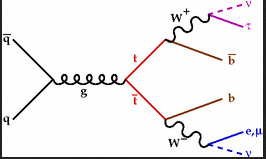
\includegraphics[width=0.7\textwidth]{figures/topAntiTopFeynDiagram.png}
	\caption{$\ttbar$ Feynman diagram \cite{ttbarDiagram}.}
	\label{fig:ttbarDiag}
\end{figure}

\begin{figure}[h]
	\centering
	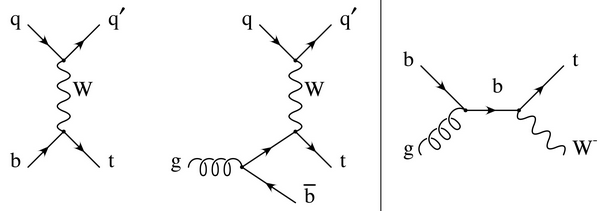
\includegraphics[width=0.7\textwidth]{figures/singleTopQuarkFeynDiagrams.png}
	\caption{Single top quark Feynman diagrams \cite{singleTopQrkDiagrams}.}
	\label{fig:singleTopDiags}
\end{figure}

The top quark background was estimated directly from collision data that passed the $e\mu$ channel requirements.  
An estimate of the pure top quark background was possible in the $e\mu$ channel for several reasons.  Based on 
the lepton flavor conservation assumption stated in Chapter \ref{sec:lrsPhenomenology}, a \WR signal produced 
events that passed the $e\mu$ channel selections at a rate suppressed by the weak coupling constant 
$g_{R} \sim \frac{1}{100}$.  In addition, the SM backgrounds without top quarks listed in Chapter \ref{sec:MC} 
produced events that passed the $e\mu$ channel selection at a rate suppressed by the electromagnetic coupling 
constant $\alpha \sim \frac{1}{100}$.  Thus, the $e\mu$ channel was expected to be dominated by top quark 
processes.  This was confirmed by comparing $e\mu$ channel data and simulations, as shown in Figure \ref{fig:dataAndSimsInEMuChannel}.

\begin{figure}[h]
	\centering
	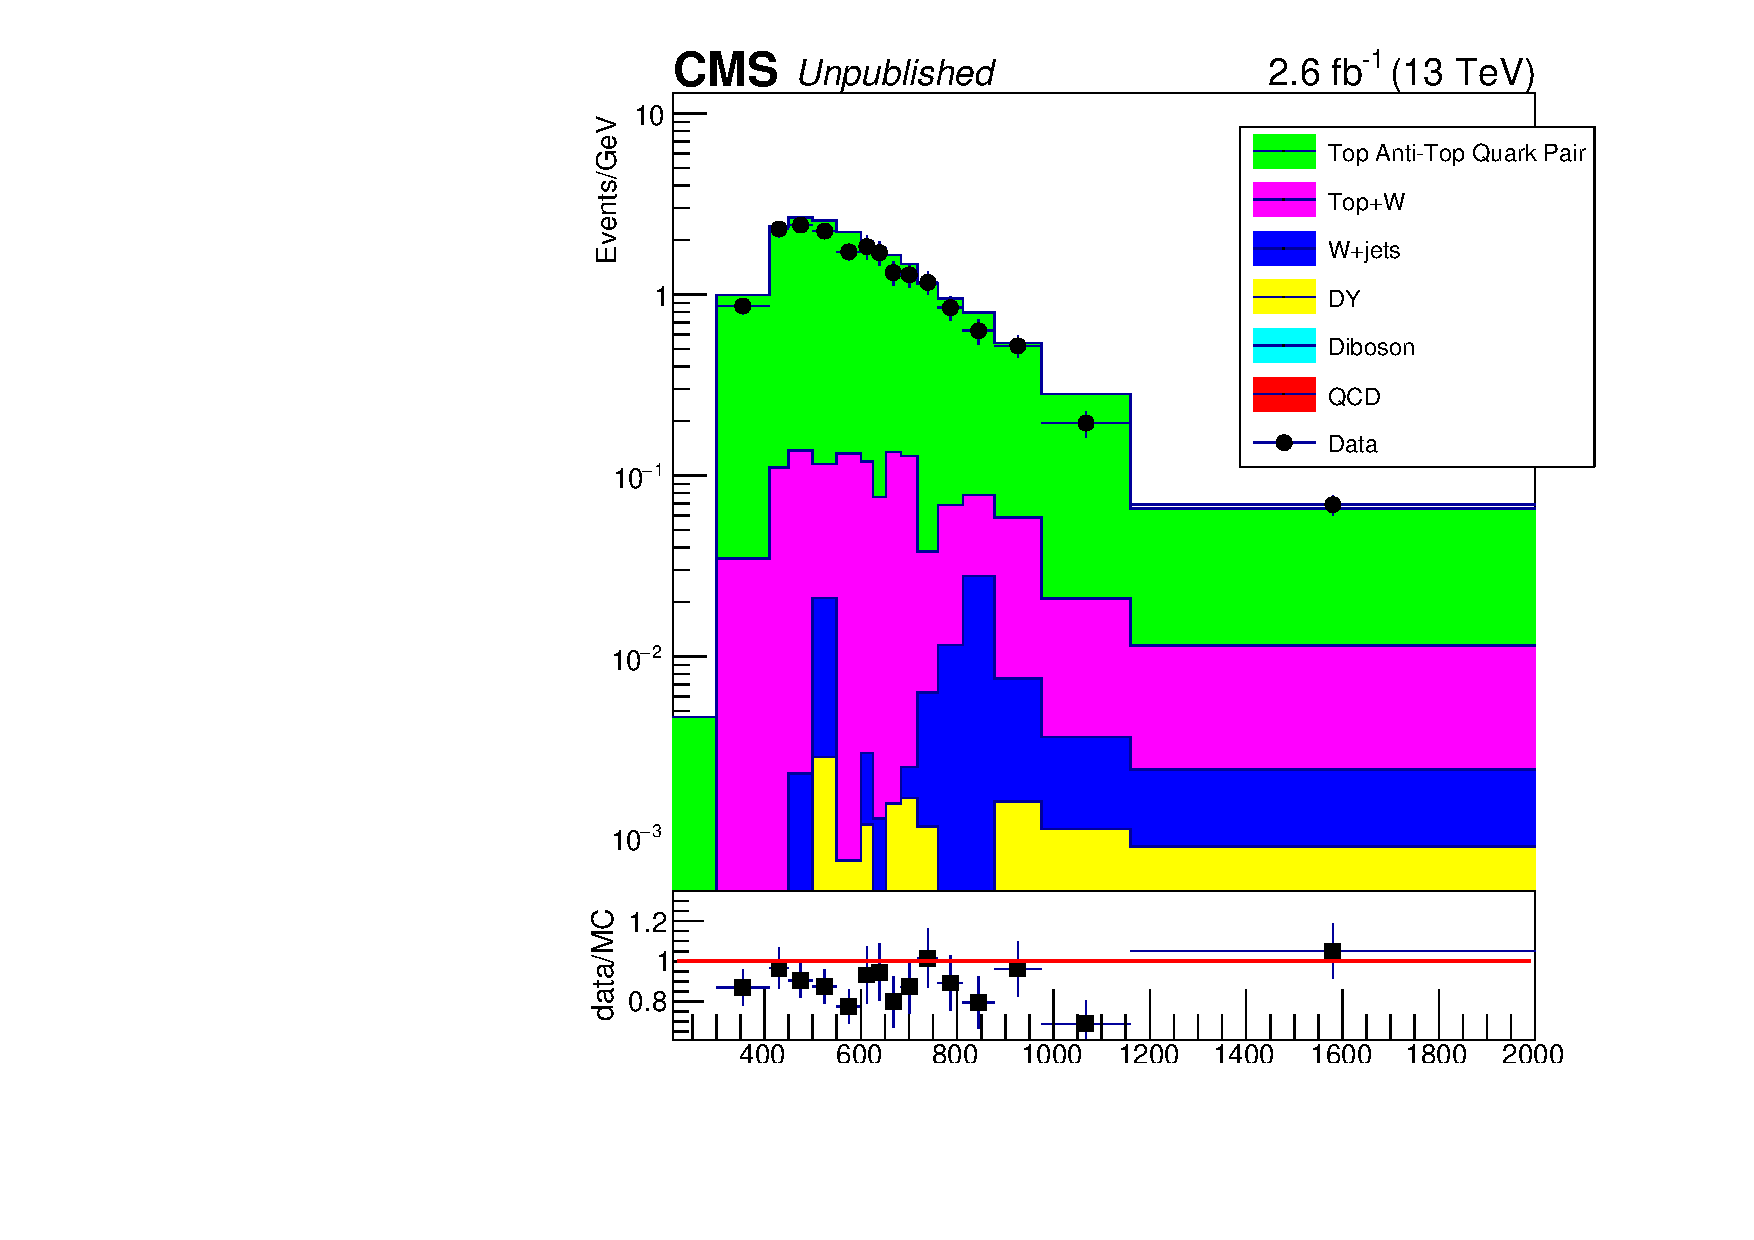
\includegraphics[width=0.7\textwidth]{figures/Mlljj_eMuChannel_log.pdf}
	\caption{The $\Mlljj$ distribution from data and simulated SM events that passed the $e\mu$ selection, excluding 
	the $\Mlljj > 600 \GeV$ cut.  The bin widths were variable, and their contents were normalized to the bin widths.}
	\label{fig:dataAndSimsInEMuChannel}
\end{figure}

To estimate the top quark background in the $eejj$ and $\mu\mu jj$ channels, scale factors (SFs) were 
calculated that scaled $e\mu jj$ data events into $eejj$ and $\mu\mu jj$ events.  The SFs were calculated using 
simulated top quark events and the following procedure:

\begin{itemize}
	\item Simulated top quark events were selected using the $ee$, $e\mu$, and $\mu\mu$ channel requirements from 
		Chapter \ref{sec:wrCandSelection}.
	\item Using selected events, the \Meejj, \Memujj and \Mmumujj distributions were produced.
	\item Using the integrals \Nemujj and \Nlljj of the \Memujj and \Mlljj distributions, the top quark background SF 
		for the $\ell\ell jj$ final state was calculated as $\Nlljj / \Nemujj$.
\end{itemize}

The SF was $0.432$ in the $ee$ channel and $0.659$ in the $\mu\mu$ channel.  The $ee$ ($\mu\mu$) channel SF 
was below (above) the expected SF of $0.5$ because electrons were reconstructed with a reduced $|\eta|$ acceptance,
and selected with lower efficiency identification requirements relative to muons.  The number of simulated top quark 
events used to calculate the SFs decreased rapidly with increasing \Mlljj, so the SFs were determined primarily by 
simulated events with $\Mlljj < 1500\GeV$.  Using SFs that did not vary with \Mlljj allowed an error to enter into the 
top quark background estimate, proportional to the fluctuations of \Mmumujj/\Memujj and \Meejj/\Memujj around the 
constant SFs versus \Mlljj in Figure \ref{fig:ttbarSFratios}.  This error was covered by assigning a 10\% uncertainty 
to both SFs.

After calculating the SFs, the top quark background in the $\mu\mu jj$ ($eejj$) final state was estimated by 
multiplying the \Memujj distribution from data by $0.659$ ($0.432$).  Based on simulations of SM backgrounds, contributions 
of non-top quark backgrounds to the $e\mu$ channel were more than one order of magnitude smaller than the 10\% top quark 
background uncertainty.  As a result, simulated non-top quark background events were not subtracted from $e\mu$ channel 
data.

\begin{figure}[btp]
	\centering
	\subfigure{
		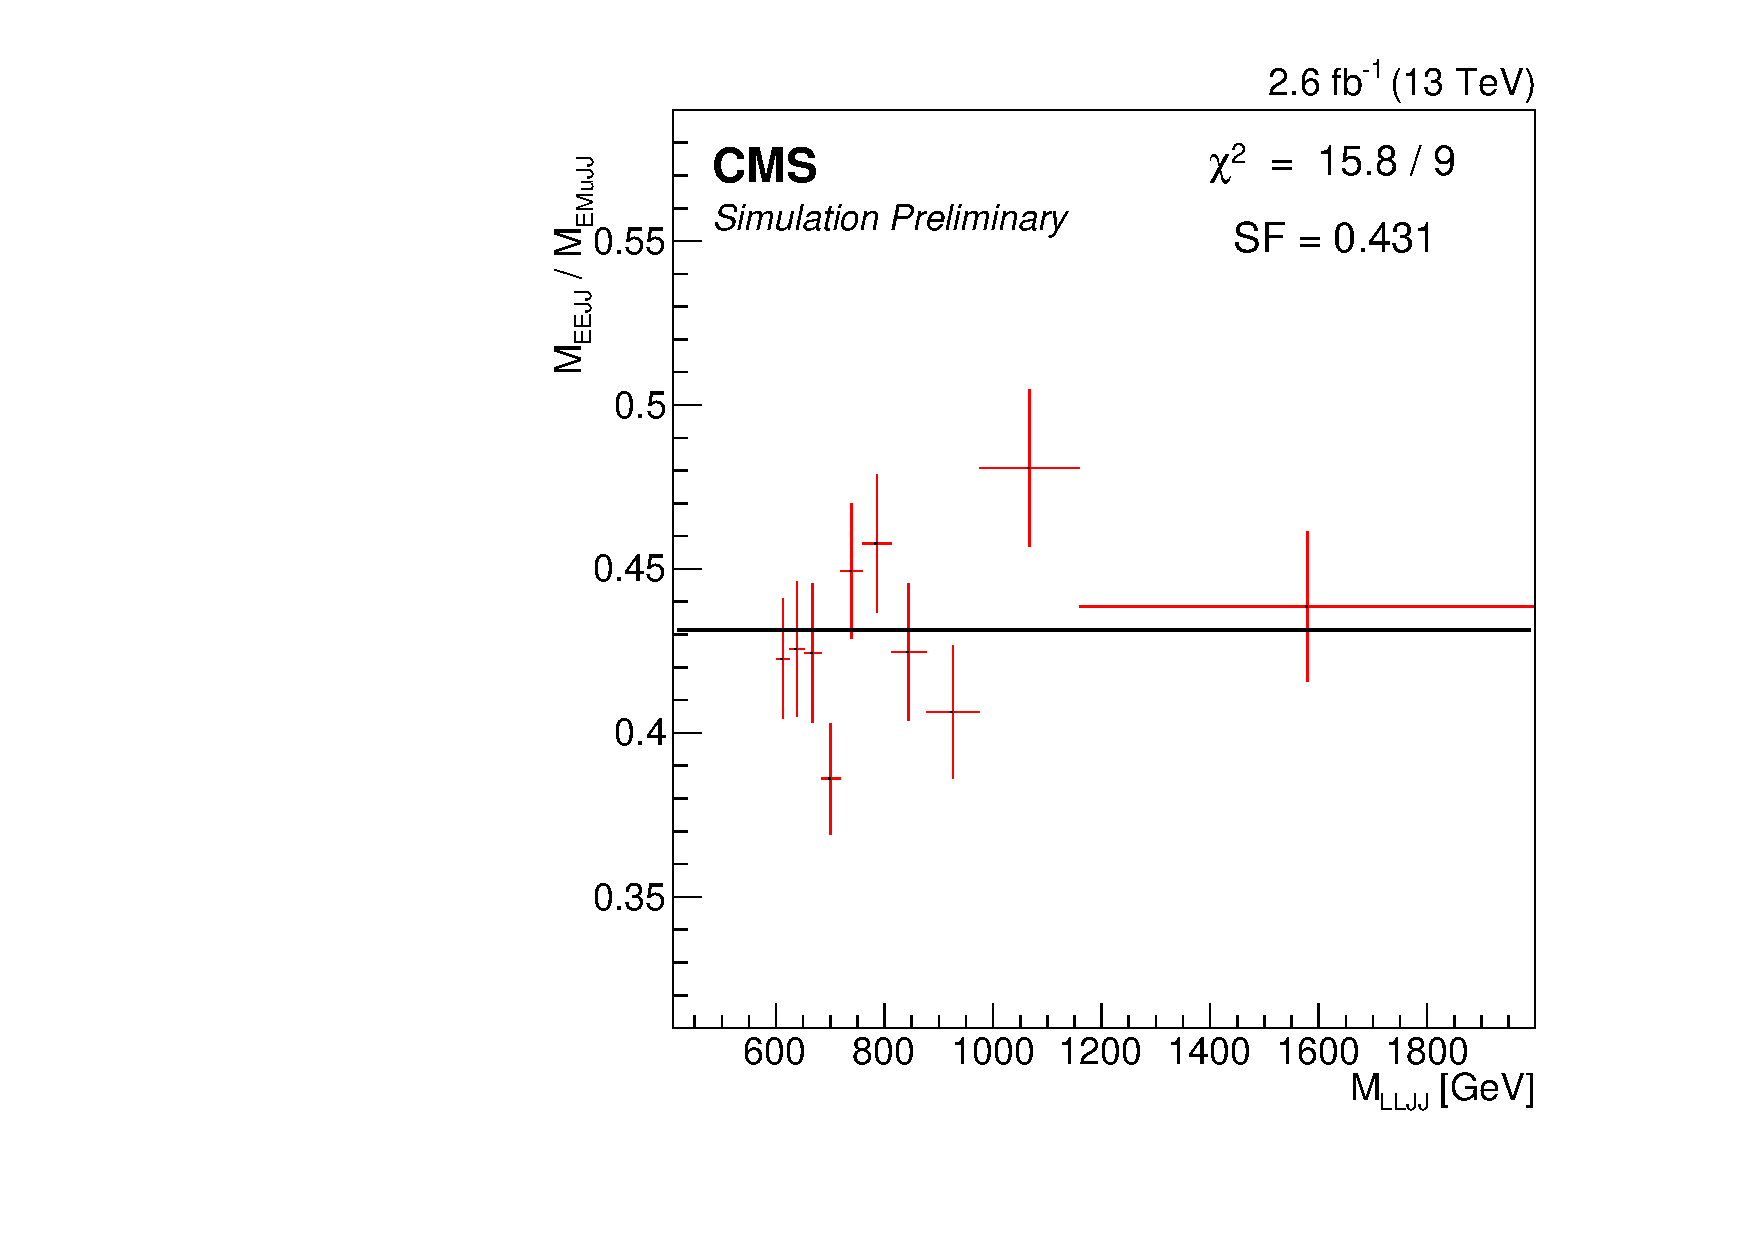
\includegraphics[width=0.45\textwidth]{figures/flavor_ratio_EE_variablebinwidth.pdf}
	}
	\subfigure{
		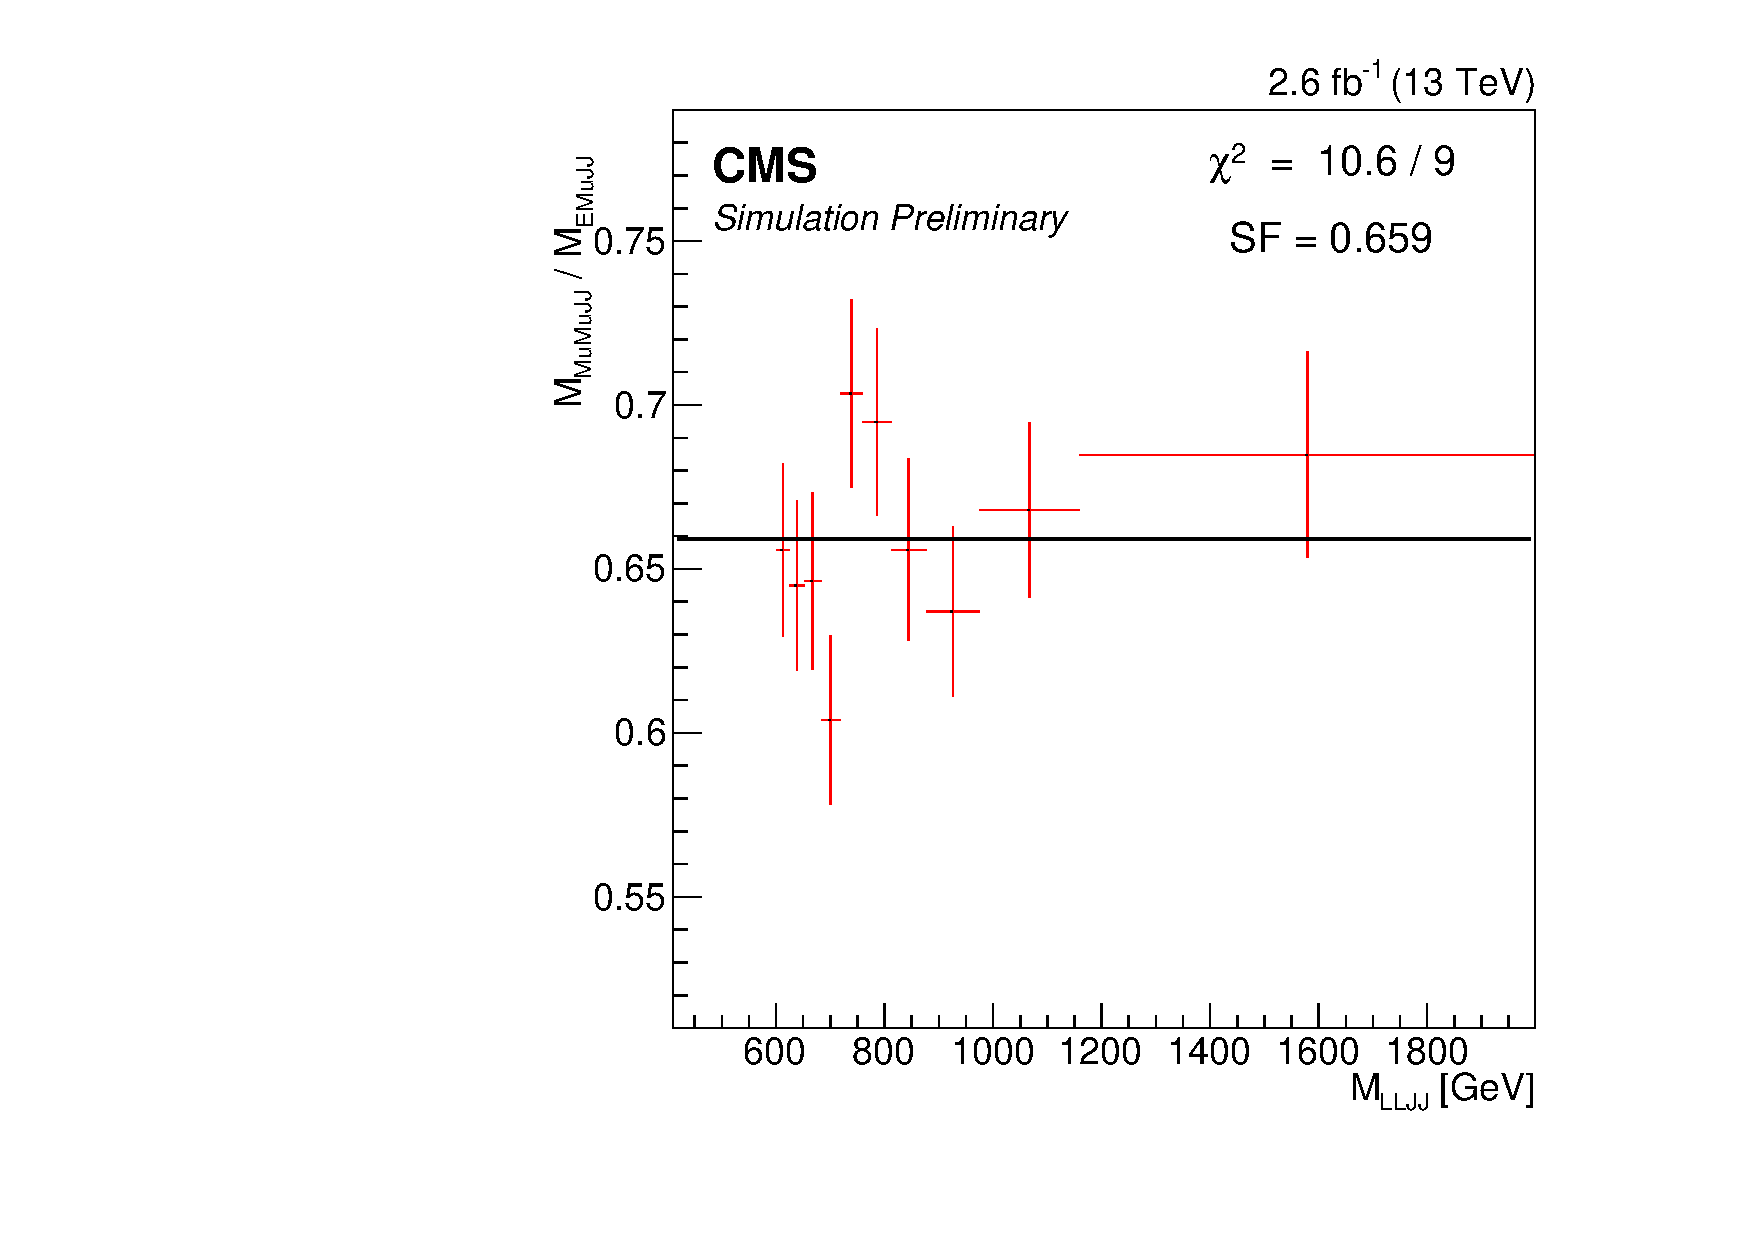
\includegraphics[width=0.45\textwidth]{figures/flavor_ratio_MuMu_variablebinwidth.pdf}
	}
	\label{fig:ttbarSFratios}
	\caption{Bin-by-bin ratio of $\Mlljj$ and $\Memujj$ distributions from simulated top quark backgrounds, where $\ell$ was 
	an electron (left) or a muon (right).}
\end{figure}


\section{\DY Background}
\label{sec:dyBkgnd}
The production and decay of Z bosons to lepton pairs in association with jets ($\DY$+jets), $pp \rightarrow Z+jets \rightarrow \ell\ell+jets$, 
was the other of the two largest backgrounds to the \WR and \nul search in the $\ell\ell jj$ final state.  The \DY 
background was estimated using simulated $\DY$+jets events.  Mis-modelling of $\DY$+jets in simulations lead to two discrepancies 
with respect to data.  The effects of mis-modelling on the signal region (defined in Chapter \ref{sec:wrCandSelection}) \DY background estimate 
were quantified and validated in three control regions where data and simulations of SM backgrounds were expected to agree.

The first discrepancy was a difference in normalization between data and \MC, caused by the cross section uncertainty in 
the simulation.  The effect of the discrepancy was estimated by comparing $Z \rightarrow \ell\ell$ events in data and 
\DY simulations, selected with the following requirements:

\begin{itemize}
	\item One of the background only triggers described in Chapter \ref{sec:triggers} was fired.
	\item At least two leptons were found with $\pt > 35 \GeV$ that passed identification selections described in 
		Chapter \ref{sec:event_selection_chapter}.  If more than two leptons were found, only the two highest $\pt$ 
		leptons were used.
	\item At least two jets were found with $\pt > 40 \GeV$ that passed identification selections.  If more than two jets 
		were found, only the two highest $\pt$ jets were used.
	\item The leptons and jets had $|\eta| < 2.4$.
	\item The two leptons had di-lepton mass $70 < M_{\ell\ell} < 110 \GeV$.
	\item Both leptons were separated from both jets by $\Delta R > 0.4$.
\end{itemize}

Using selected events, the $\Mll$ distribution was made and used to compare data to simulations.  Based on simulations 
of non-\DY backgrounds, 3\% of the selected events in data came from non-\DY processes.  The effect of subtracting 
simulated non-\DY events from data was much smaller than the total uncertainty on the \DY background 
estimate, so non-\DY backgrounds were not subtracted from data.  The normalization of the $\Mll$ distribution using 
data events exceeded that of simulated events by 15.7\% in the $ee$ channel, and 14.2\% in the $\mu\mu$ channel.  To 
correct the normalization discrepancy, the \DY background estimate derived from simulated events in the signal region 
and other control region was scaled up by $\sim$15\%.

Two additional $\DY$+jets datasets, simulated with different generators for the first simulation step, were used to 
estimate the uncertainty on the $\sim$15\% correction to the \DY background predicted by simulations.  The $Z \rightarrow \ell\ell$ 
selection described earlier without jet requirements was applied to data and all three simulated $\DY$+jets datasets.  
The jet requirements were removed to compare data to simulations in a phase space where all three simulated datasets 
yielded a large number of events after selections.  Using selected events, the difference in normalization between data and 
simulations in the $\Mll$ distribution was calculated, and the largest difference was taken as a systematic 
uncertainty on $\sim$15\%.  This uncertainty was estimated to be 2.0\% (1.0\%) in the $ee$ ($\mu\mu$) channel.

Unlike the jets produced naturally as a result of quark decay in $\ttbar \rightarrow \ell\ell jj$ events, jets 
produced in \DY events were produced randomly by the strong interaction, sometimes before the Z boson was produced.  Simulations of random 
jet production in \DY events were done only at leading order in the strong interaction, and as a result 
the $\pt, \eta, \phi$ of jets predicted by simulations did not perfectly agree with jets observed in data.  This disagreement 
created the second discrepancy between data and simulated \DY, which manifested as a difference in $\Mlljj$ shape.  
The effect of the $\Mlljj$ shape disagreement was estimated using data and simulations of SM backgrounds selected 
with the signal region requirements described in Chapter \ref{sec:wrCandSelection}, but with $\Mll < 180 \GeV$.  Subsequently, 
$\Mlljj$ distributions were built from selected data and all simulated events, and the \DY component of selected simulated events was 
rescaled by $1.157$ ($1.142$) in the $ee$ ($\mu\mu$) channel to correct for the normalization discrepancy discussed 
previously.  Then, the $\Mlljj$ distributions from data and simulations shown in 
Figure \ref{fig:mlljjLowDileptonMassSideband} were compared, and the largest percentage difference between data and 
all simulations in any bin was taken as a conservative systematic uncertainty on the estimated \DY background.  The 
mis-modelling of jets in simulations resulted in a symmetric 40\% uncertainty assigned to the \DY background in both channels, 
constant versus $\Mlljj$.

\begin{figure}[btp]
\centering
\subfigure{
  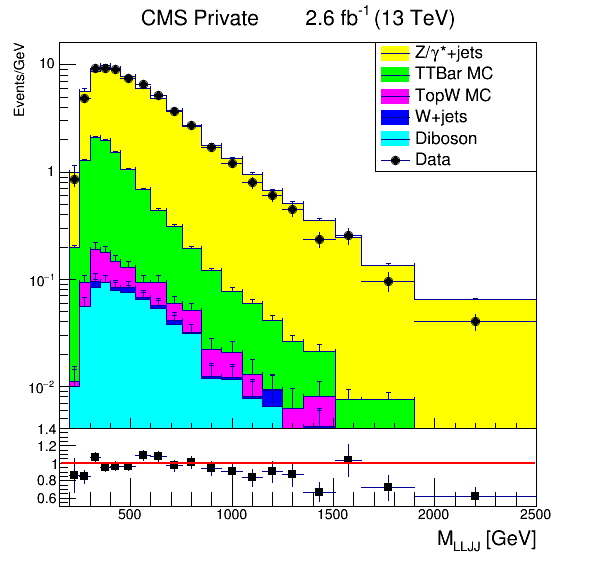
\includegraphics[width=0.45\textwidth]{figures/Mlljj_eeChnl_lowMllCR.png}
}
\subfigure{
  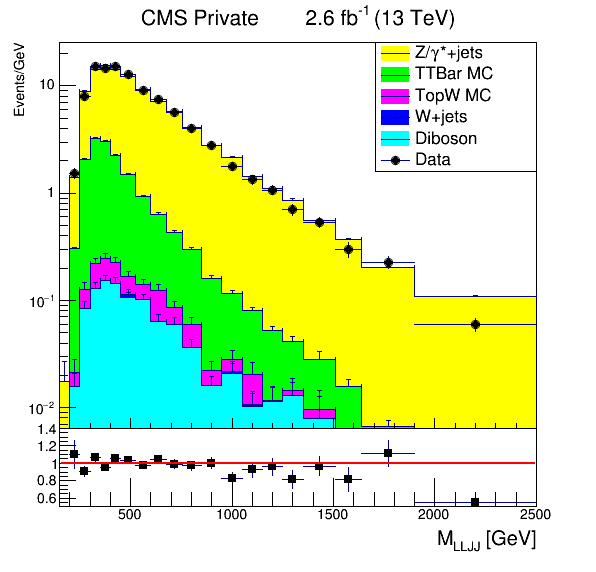
\includegraphics[width=0.45\textwidth]{figures/Mlljj_mumuChnl_lowMllCR.png}
}
\caption{The $\Mlljj$ distribution from data and simulated SM events that passed the $\Mll < 180 \GeV$ selection, the 
		$ee$ ($\mu\mu$) channel on the left (right).  The bin widths were variable, and their contents were normalized to 
	the bin widths.}
\label{fig:mlljjLowDileptonMassSideband}
\end{figure}

In an attempt to reduce the 40\% uncertainty, a separate set of simulated $\DY$+jets events were used, in which jet simulations 
were done at a higher order in the strong interaction.  By simulating jet production at a higher order in the strong 
interaction, it was thought that the disagreement in $\Mlljj$ shape could be reduced.  The results, shown in Figure 
\ref{fig:mlljjLowDileptonMassSidebandAMCNLO}, did not support switching simulated \DY datasets.  The primary detriment to the 
higher order \DY simulation was not the jet simulation, but the lack of events.  After selections, the leading order 
simulated $\DY$+jets dataset had $\sim$3 times more events across all $\Mlljj$, and $\sim$10 times more events with $\Mlljj > 1 \TeV$ 
than the higher order simulated $\DY$+jets dataset.

\begin{figure}[btp]
\centering
\subfigure{
  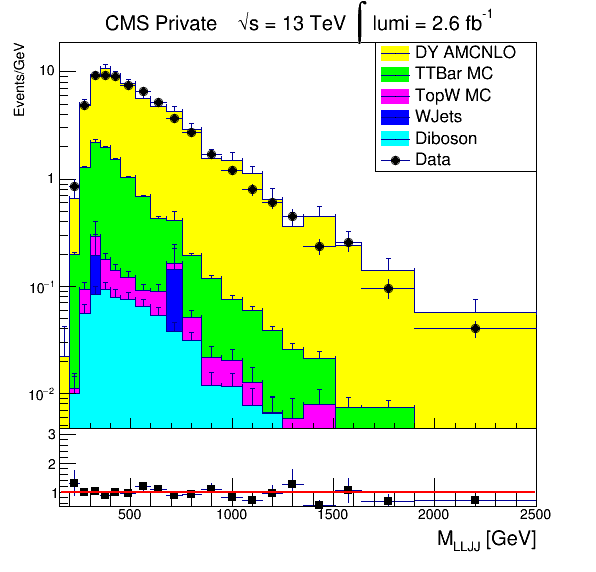
\includegraphics[width=0.45\textwidth]{figures/Mlljj_eeChnl_lowMllCR_AMCNLO.png}
}
\subfigure{
  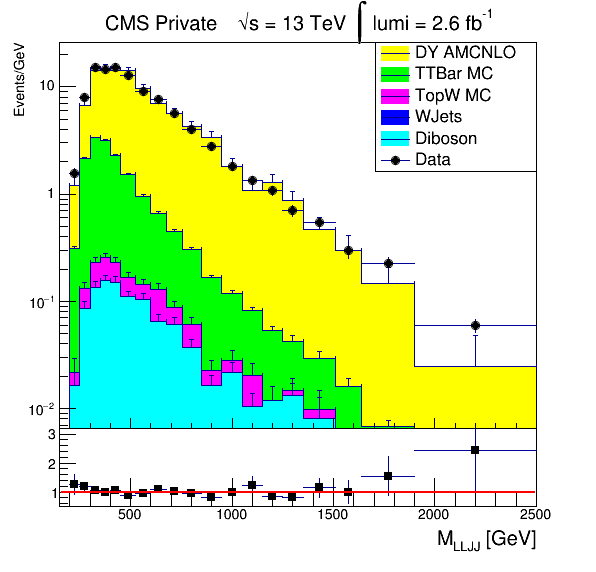
\includegraphics[width=0.45\textwidth]{figures/Mlljj_mumuChnl_lowMllCR_AMCNLO.png}
}
\caption{The $\Mlljj$ distribution from data and simulated SM events that passed the $\Mll < 180 \GeV$ selection, the 
		$ee$ ($\mu\mu$) channel on the left (right).  The bin widths were variable, and their contents were normalized to 
	the bin widths.  In the \DY events, jet production was simulated at a higher order relative to the standard \DY dataset.}
\label{fig:mlljjLowDileptonMassSidebandAMCNLO}
\end{figure}

A third control region was used to validate the correction applied and uncertainty assigned to the estimated \DY background.  
In this control region, events from data and simulations of all SM backgrounds were selected with 
the signal region requirements described in Chapter \ref{sec:wrCandSelection}, but with $\Mlljj < 600 \GeV$.  Selected 
data and simulated events were used to make an $\Mll$ distribution, and the simulated \DY component was rescaled 
by $\sim1.15$.  Based on comparisons between data and simulations shown in Figure \ref{fig:mllInLowMlljjSideband}, the 
correction applied to simulated \DY events brought data and simulations of SM backgrounds into better agreement.  In addition, 
the uncertainty assigned to simulated \DY allowed the estimated \DY background to float in a range that improved the overall 
agreement between data and simulations.

\begin{figure}[btp]
\centering
\subfigure{
  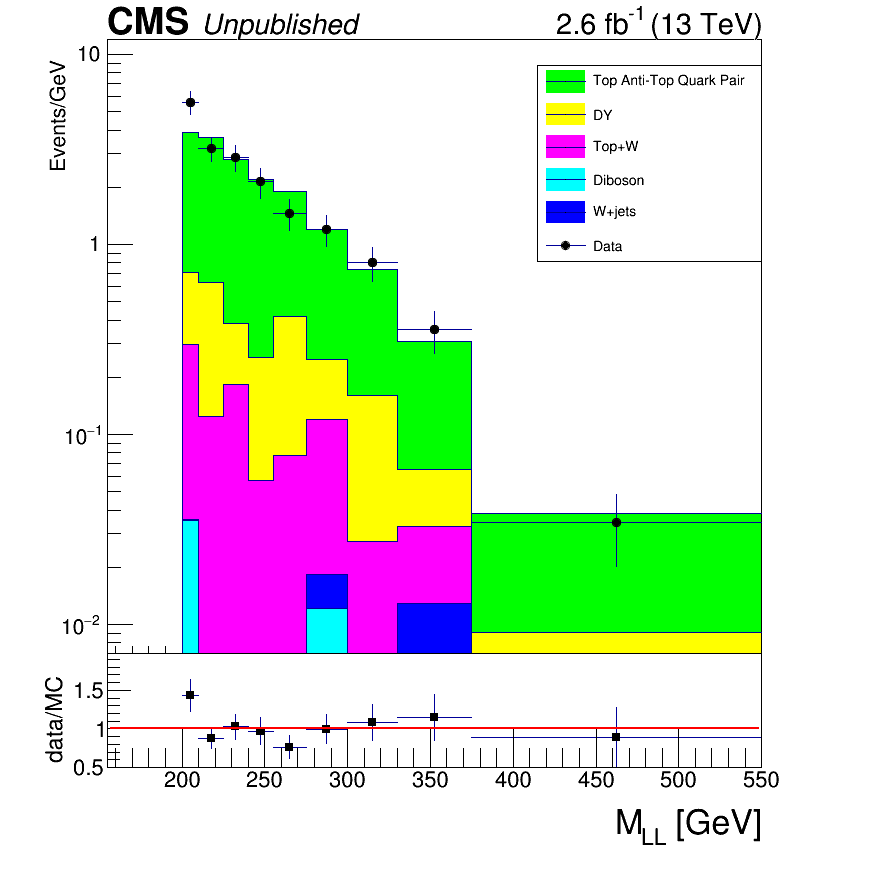
\includegraphics[width=0.45\textwidth]{figures/Mll_eeChnl_lowMlljjCR.png}
}
\subfigure{
  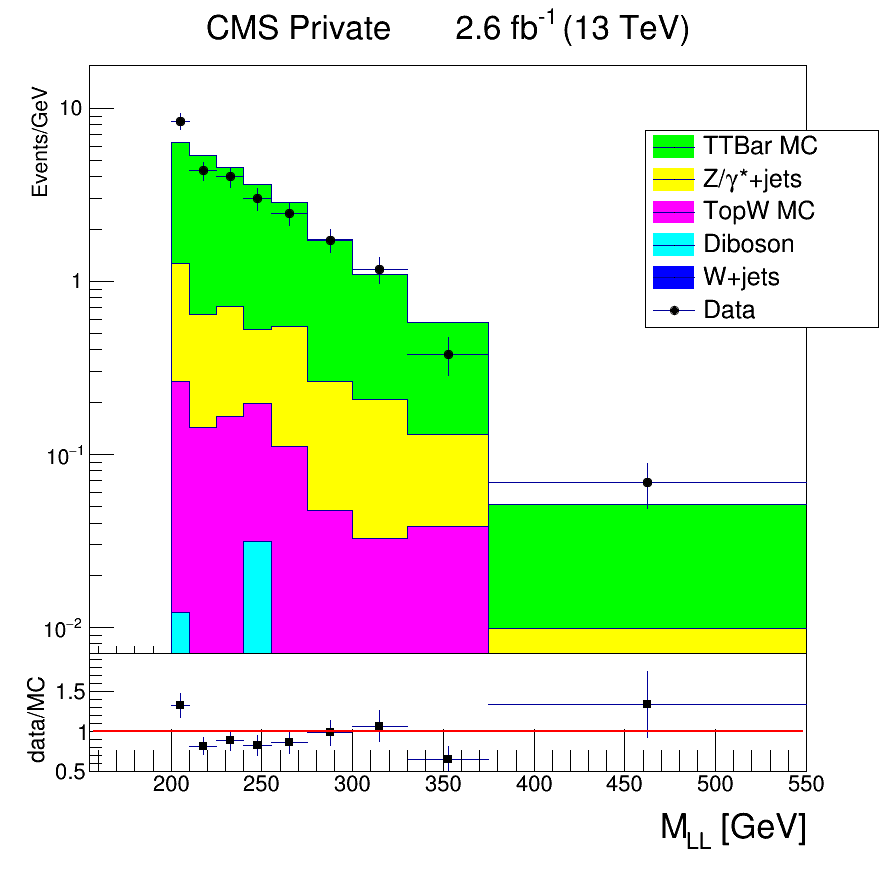
\includegraphics[width=0.45\textwidth]{figures/Mll_mumuChnl_lowMlljjCR.png}
}
\caption{$\Mll$ for data and simulations of all SM backgrounds in the $\Mlljj < 600\GeV$ control region.  The 
$ee$ ($\mu\mu$) channel was on the left (right).}
\label{fig:mllInLowMlljjSideband}
\end{figure}

The \DY background was estimated by selecting simulated \DY events with the signal region selections described in Chapter 
\ref{sec:wrCandSelection}.  The weight of selected events were scaled by 1.157 (1.142) in the $ee$ ($\mu\mu$) channel, and 
the scaled events represented the estimated \DY background.  Based on comparisons between data and simulated \DY events in 
control regions, a 40\% uncertainty for all $\Mlljj > 600\GeV$ was assigned to the estimated \DY background.


\section{Diboson and W+jets Backgrounds}
\label{sec:dibosonAndWJetsBkgnds}
The production of weak boson $W/Z$ pairs (WW, WZ, ZZ), and single W bosons in association with jets yielded events where 
two charged leptons and two jets were reconstructed and passed the signal region selections.  The number of events in 
data produced by these processes was estimated using simulated W+jets and diboson events.  The expected number of events from diboson and W+jets 
processes, shown in Figure \ref{fig:allExpectedBkgnds}, was small relative to \DY and top quark backgrounds, and concentrated 
in the region $\Mlljj < 2000\GeV$.  The diboson and W+jets processes were neglected when calculating final results for 
this search.

\begin{figure}[h]
	\centering
	\subfigure{
		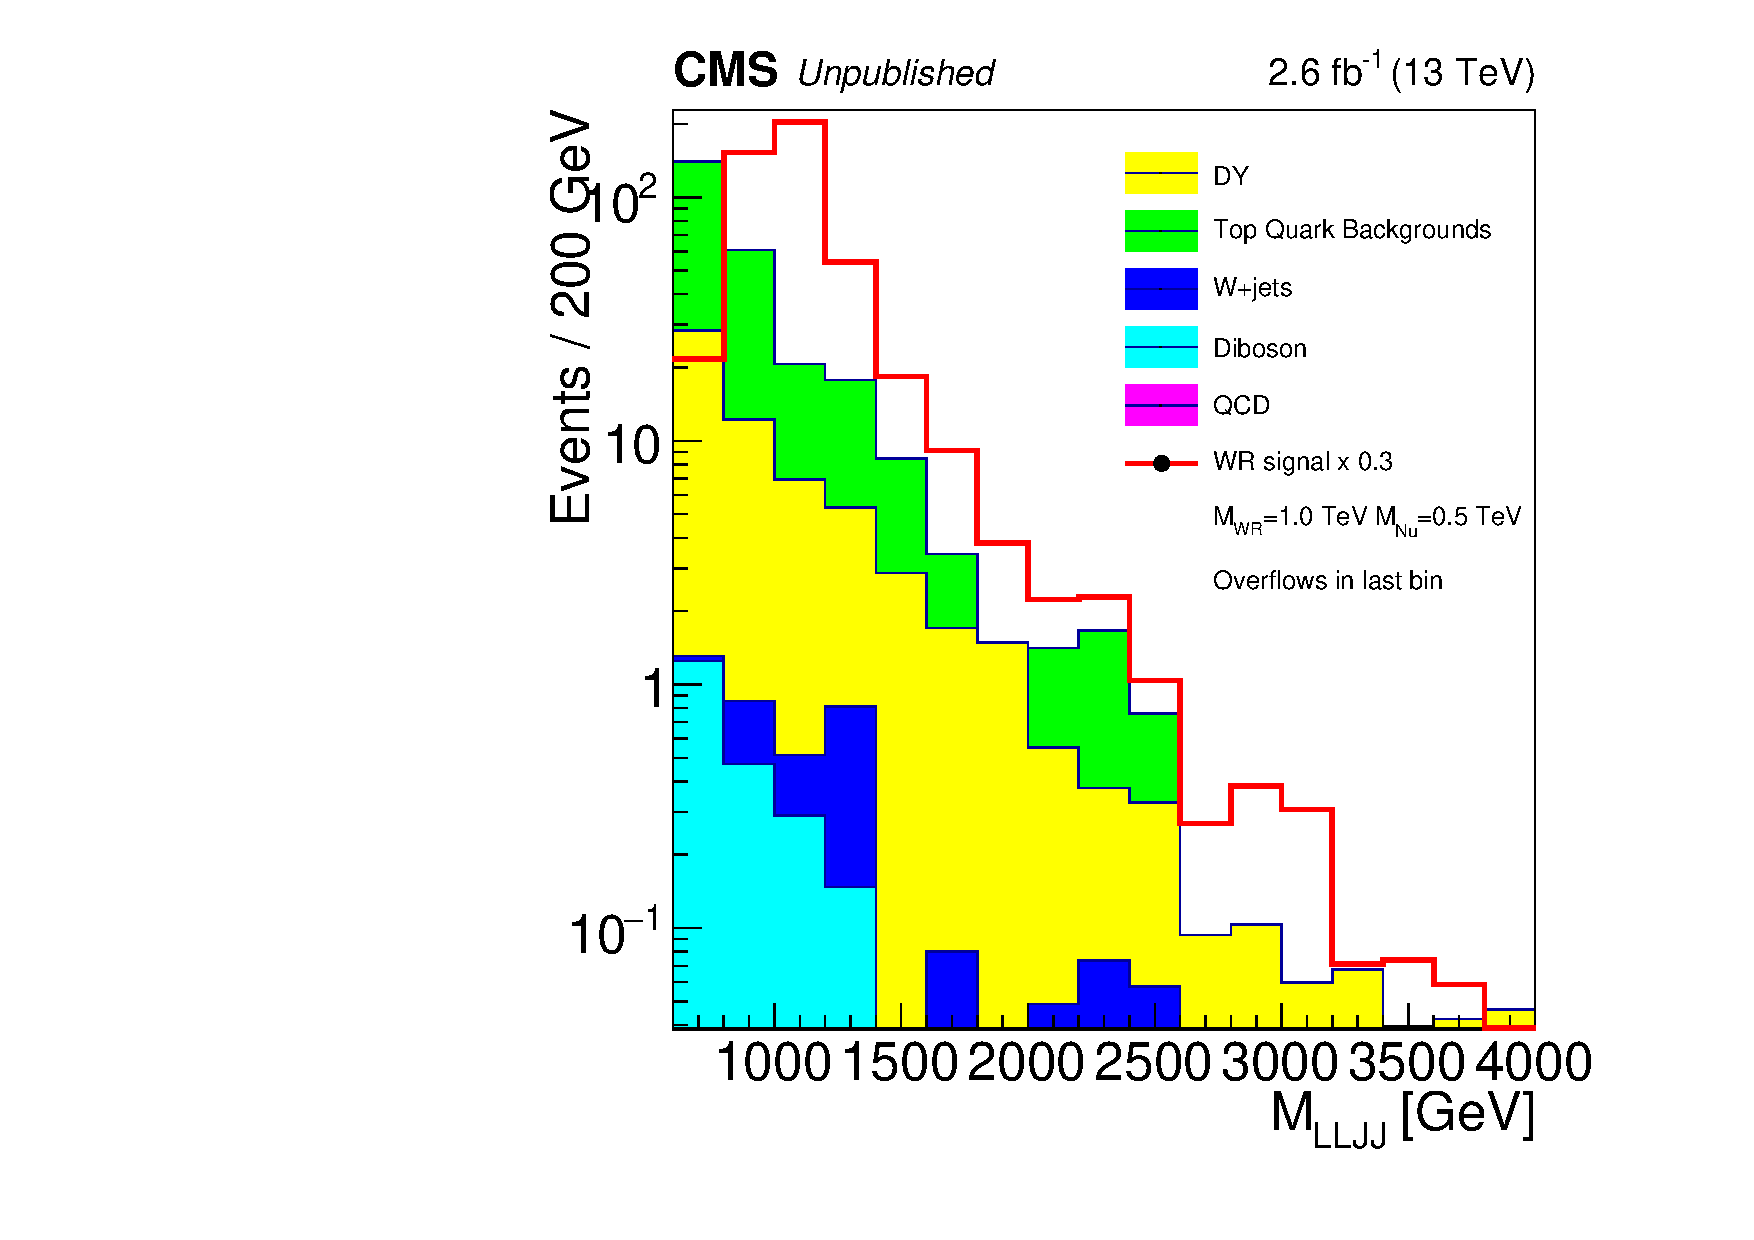
\includegraphics[width=0.45\textwidth]{figures/useOfLLJJMassAsFigureOfMerit.pdf}
	}
	\subfigure{
		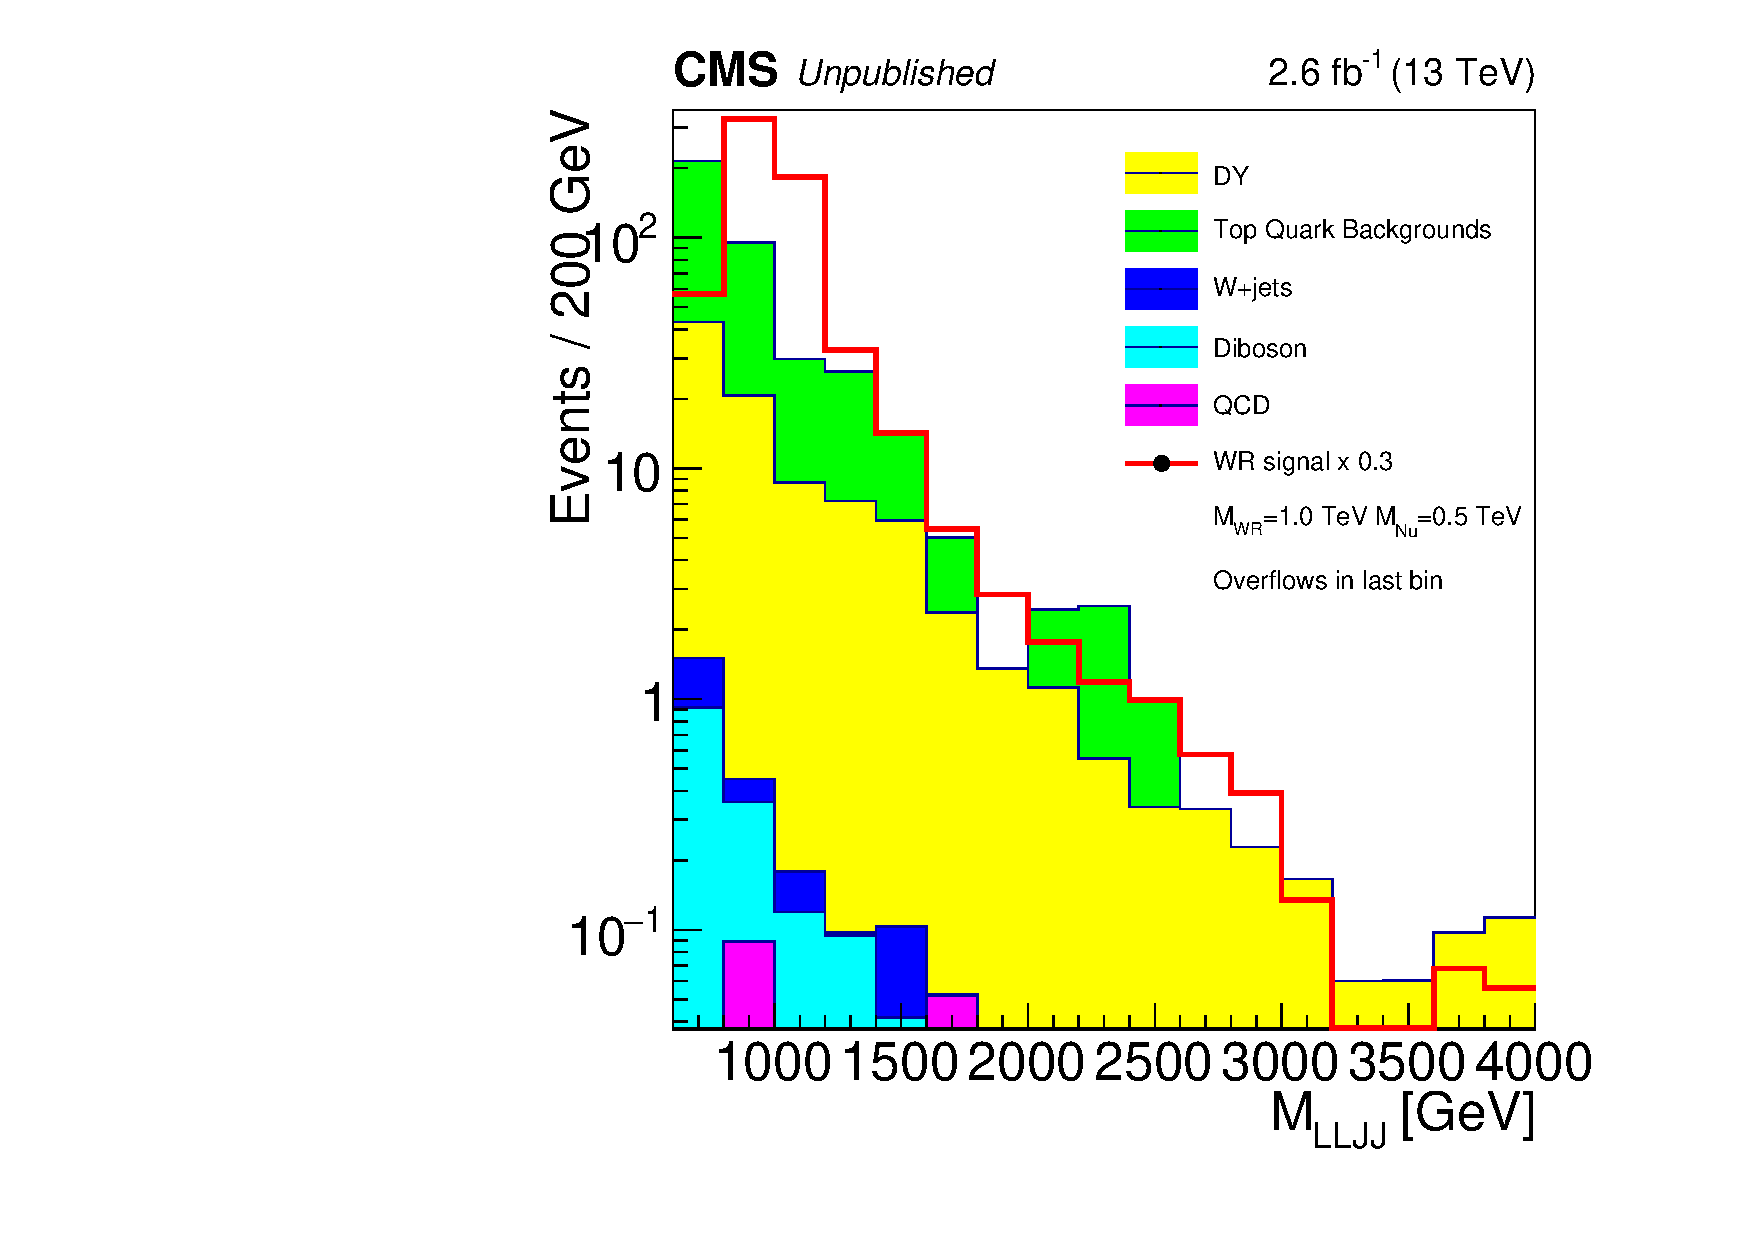
\includegraphics[width=0.45\textwidth]{figures/Mlljj_mumuChnl_signalRegionNoData.pdf}
	}
	\label{fig:allExpectedBkgnds}
	\caption{$\Mlljj$ distributions from simulated \DY, diboson, W+jets backgrounds, and the top quark and QCD backgrounds estimated from 
		data. The normalization of the \WR $\Mlljj$ distribution was scaled down by 70\% to facilitate comparisons between expected 
		signal and backgrounds.  The $ee$ ($\mu\mu$) channel was shown on the left (right).}
\end{figure}


\section{QCD Background}
\label{sec:qcdBkgnd}
The production of jets through QCD processes yielded multi-jet events where two charged leptons and two jets were reconstructed 
and passed the signal region selections.  In such events, two real jets were incorrectly reconstructed and identified as charged 
leptons.  The QCD multi-jet background expected in data was estimated by first selecting events in data with the signal region requirements 
described in Chapter \ref{sec:wrCandSelection}, but with looser identification selections applied to lepton candidates.  Events where one 
or both selected leptons passed the standard lepton identification selections were discarded, as these selected leptons were most likely 
real charged leptons.  Then, remaining events were weighted by the probability for both selected leptons, which most likely 
originated from jets, to pass the standard lepton identification requirements.  This probability was determined in an independent 
sample of data and simulated events as a function of $\eta$ and $\pt$ or $\Et$ of leptons that were incorrectly reconstructed from 
real jets.  After the probability weights were applied to selected events, the contribution of weighted events to the $\Mlljj$ 
distribution was compared to the $\Mlljj$ distribution expected from other SM backgrounds, shown in Figure \ref{fig:allExpectedBkgnds}.  
The expected QCD background was negligible, and was ignored when calculating final results for this search.


%%%%%%%%%%%%%%%%%%%%%%%%%%%%%%%%%%%%%%%%%%%%%%%%%%%%%%%%%%%%%%%%%%%%%%%%%%%%%%%%
